\begin{figure}[!hp]
  \begin{center}
      \begin{tikzpicture}
        \begin{axis}[
            %colorbar,
            hide axis,
            scale only axis,
            height=0.26\rasterimagewidth,,
            width=\rasterimagewidth,
            %colorbar horizontal,
            point meta min=2.43,
            point meta max=3.05,
            colorbar style={
              title=Concentration [\%w],
              width=7.4cm,
              height=0.3cm,
              xtick={2.43,2.5,2.75, 3, 3.05, 3.5, 4, 4.5, 5, 5.5, 6},
              at={(0.5\rasterimagewidth,0.4cm)},
              anchor=north
            }
          ]
          \addplot [] coordinates {(0,0)};
          \node (myfirstpic) at (0,0) {\framebox{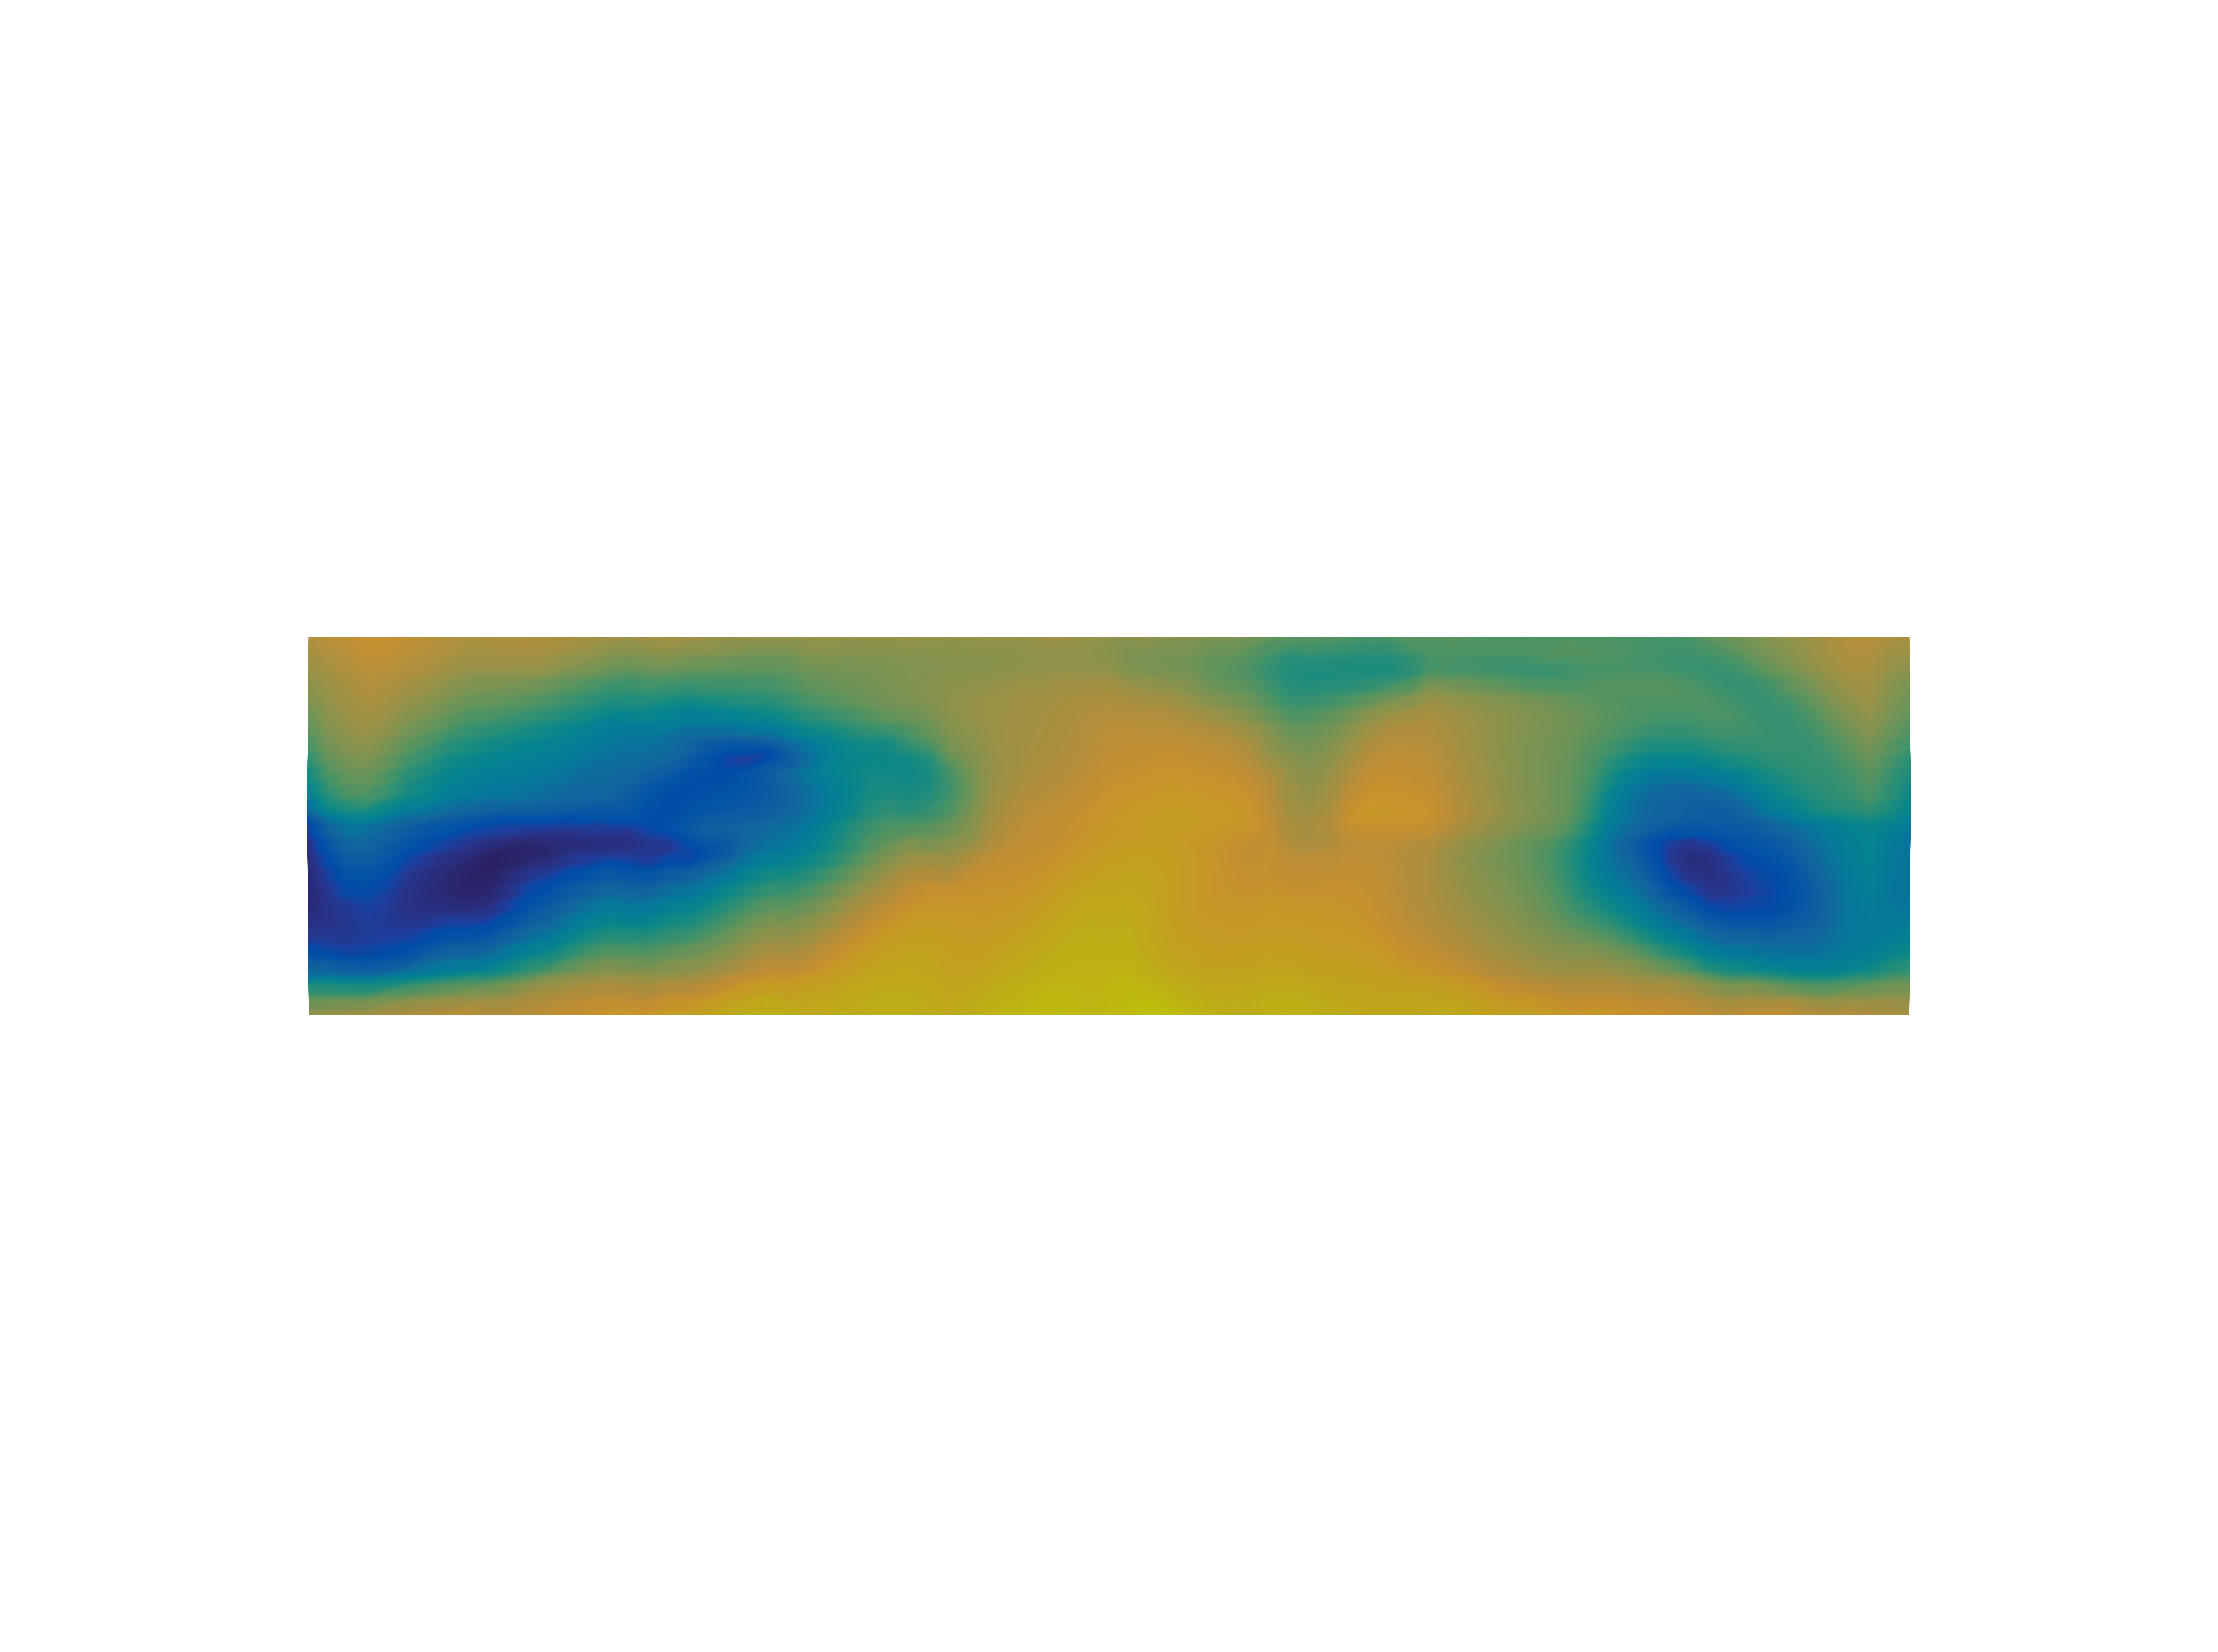
\includegraphics[width=\rasterimagewidth]{{../media/populations/application/print/alumina-influance-sur1-2.43-3.05}.png}}};
        \end{axis}
      \end{tikzpicture}
      \begin{tikzpicture}
        \begin{axis}[
            %colorbar,
            hide axis,
            scale only axis,
            height=0.26\rasterimagewidth,,
            width=\rasterimagewidth,
            %colorbar horizontal,
            point meta min=2.51,
            point meta max=3.02,
            colorbar style={
              title=Concentration [\%w],
              width=7.4cm,
              height=0.3cm,
              xtick={2.51,2.75, 3,3.02, 3.5, 4, 4.5, 5, 5.5, 6},
              at={(0.5\rasterimagewidth,0.4cm)},
              anchor=north
            }
          ]
          \addplot [] coordinates {(0,0)};
          \node (myfirstpic) at (0,0) {\framebox{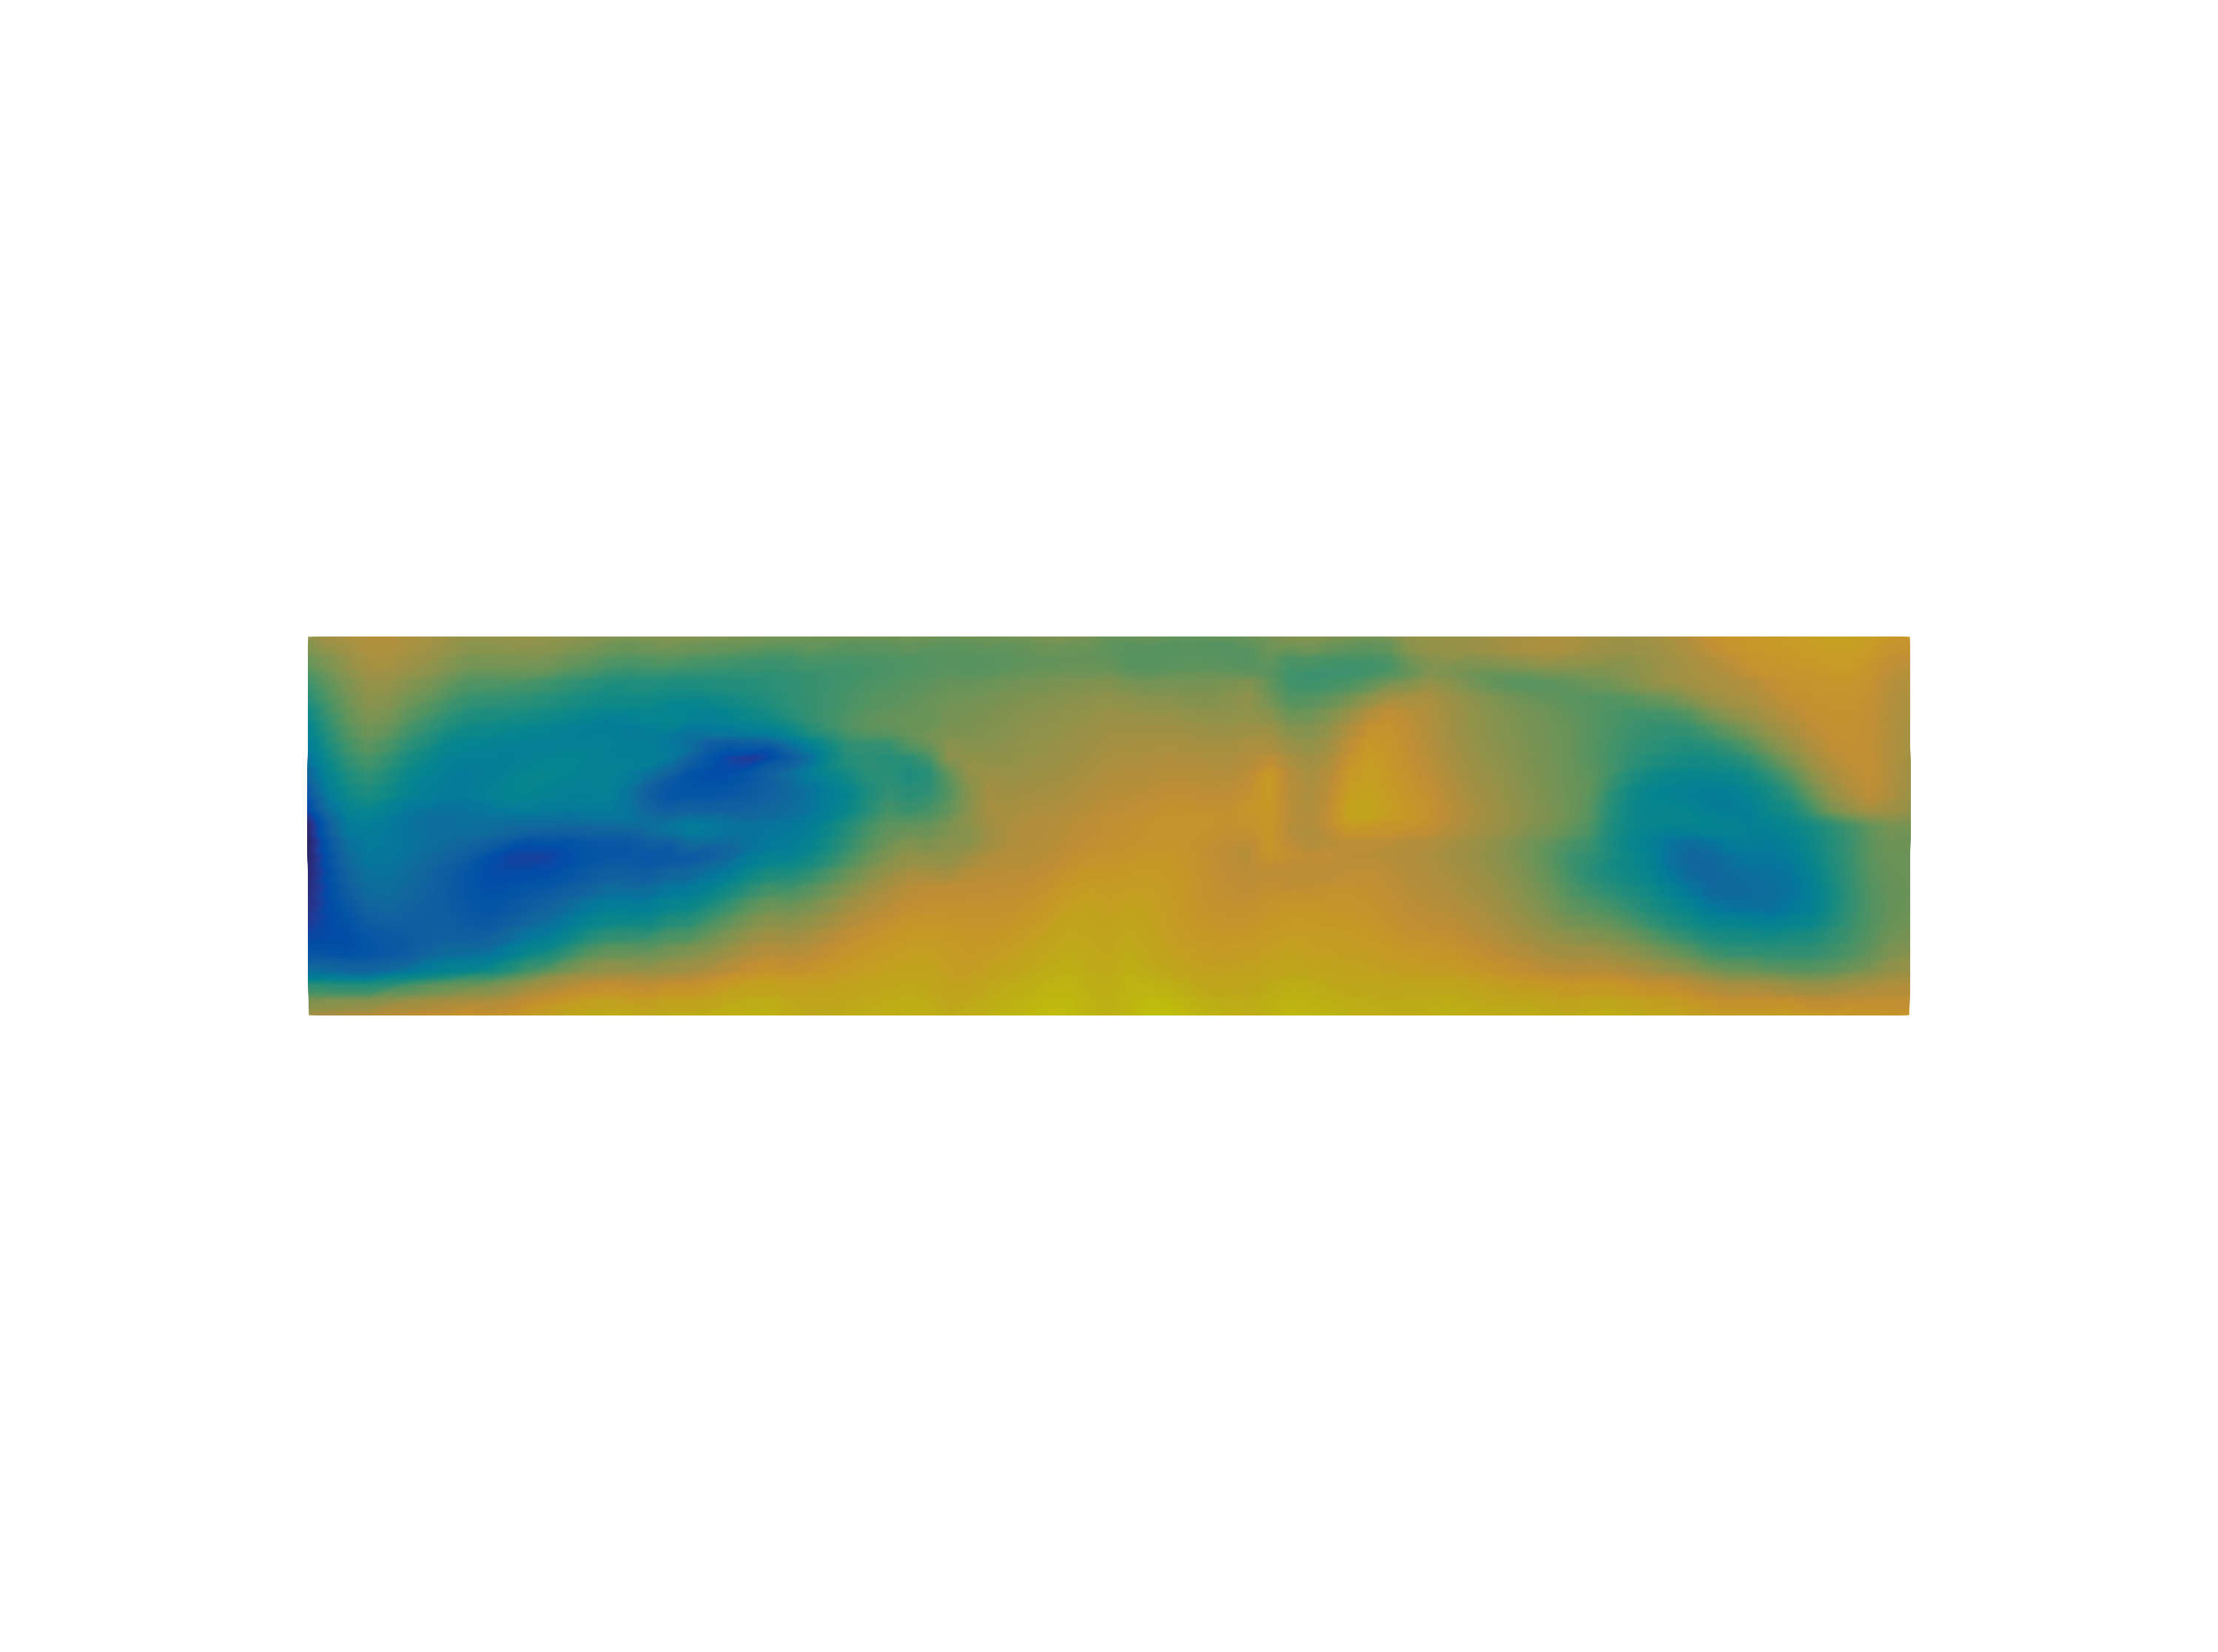
\includegraphics[width=\rasterimagewidth]{{../media/populations/application/print/alumina-influance-sur2-2.51-3.02}.png}}};
        \end{axis}
      \end{tikzpicture}
      \begin{tikzpicture}
        \begin{axis}[
            %colorbar,
            hide axis,
            scale only axis,
            height=0.26\rasterimagewidth,,
            width=\rasterimagewidth,
            %colorbar horizontal,
            point meta min=2.51,
            point meta max=3.13,
            colorbar style={
              title=Concentration [\%w],
              width=7.4cm,
              height=0.3cm,
              xtick={2.51,2.75, 3,3.13, 3.5, 4, 4.5, 5, 5.5, 6},
              at={(0.5\rasterimagewidth,0.4cm)},
              anchor=north
            }
          ]
          \addplot [] coordinates {(0,0)};
          \node (myfirstpic) at (0,0) {\framebox{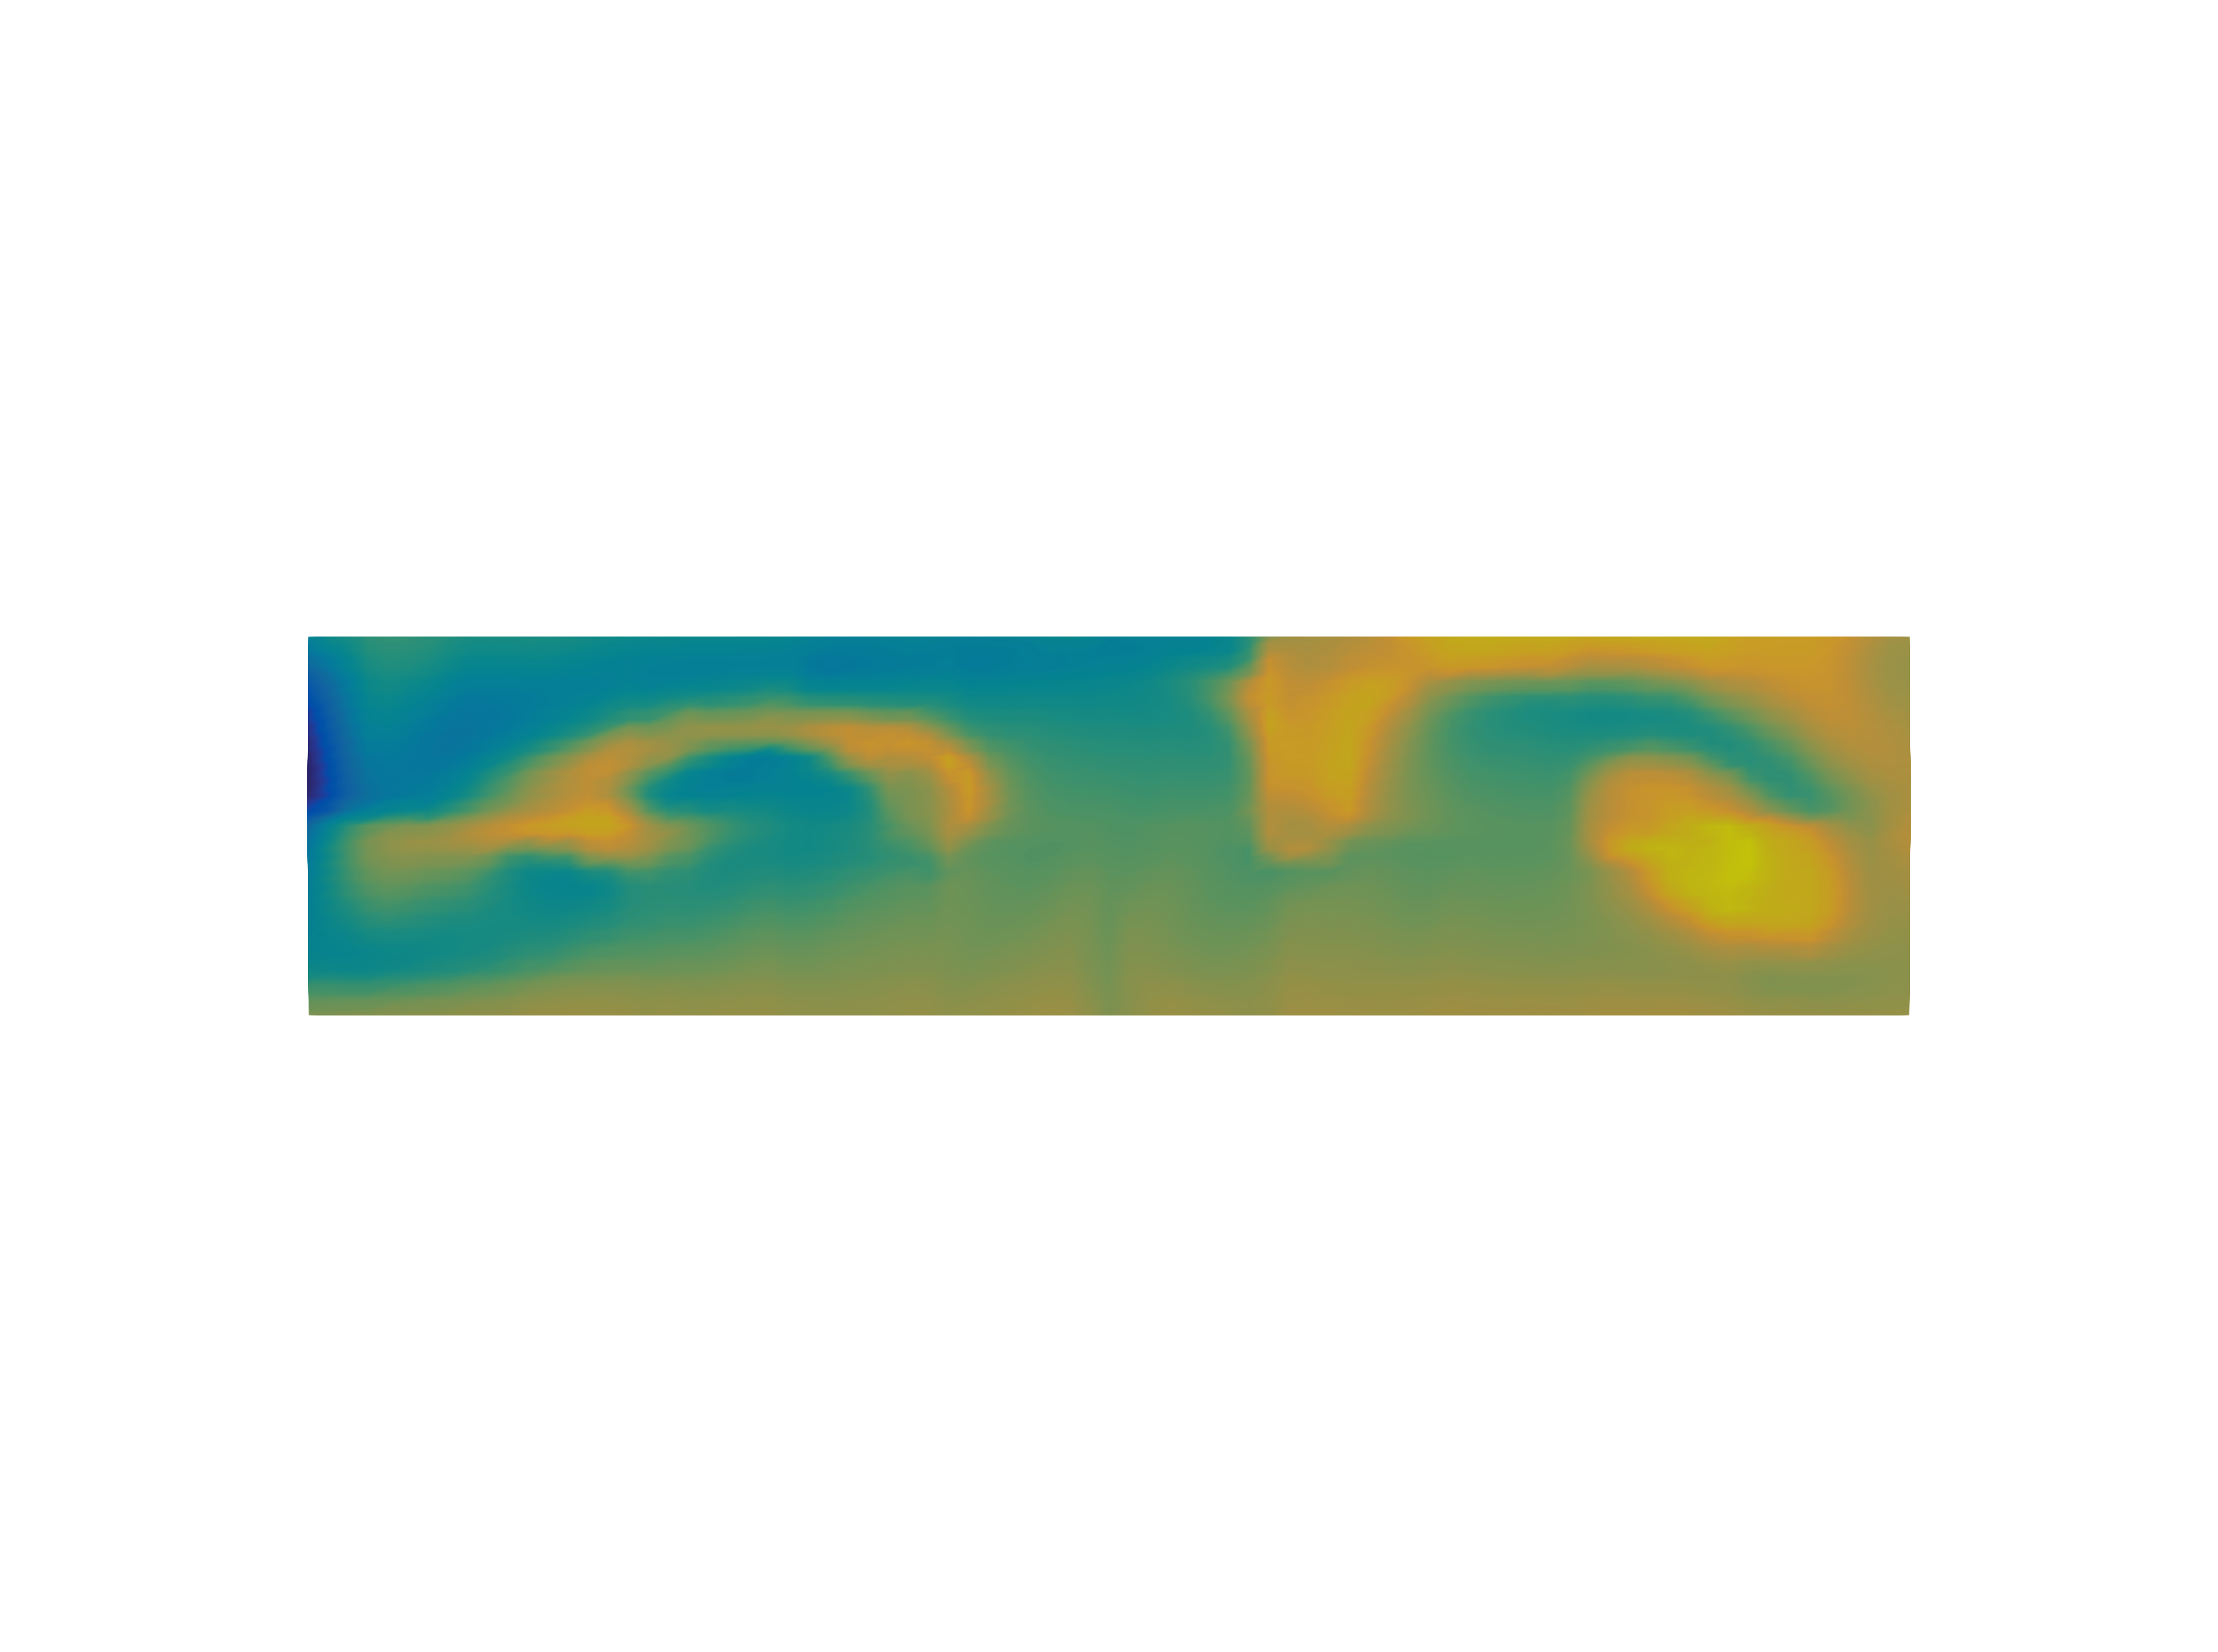
\includegraphics[width=\rasterimagewidth]{{../media/populations/application/print/alumina-influance-sur5-2.51-3.13}.png}}};
        \end{axis}
      \end{tikzpicture}
      \begin{tikzpicture}
        \begin{axis}[
            colorbar,
            hide axis,
            scale only axis,
            height=0.52\rasterimagewidth,,
            width=\rasterimagewidth,
            colorbar horizontal,
            point meta min=2.51,
            point meta max=3.13,
            colorbar style={
              title=Concentration [\%w],
              width=7.4cm,
              height=0.3cm,
              xtick={2.51, 2.75, 3, 3.13, 3.5, 4, 4.5, 5, 5.5, 6},
              at={(0.5\rasterimagewidth,3.0cm)},
              anchor=north
            }
          ]
          \addplot [] coordinates {(0,0)};
          \node (myfirstpic) at (0,50) {{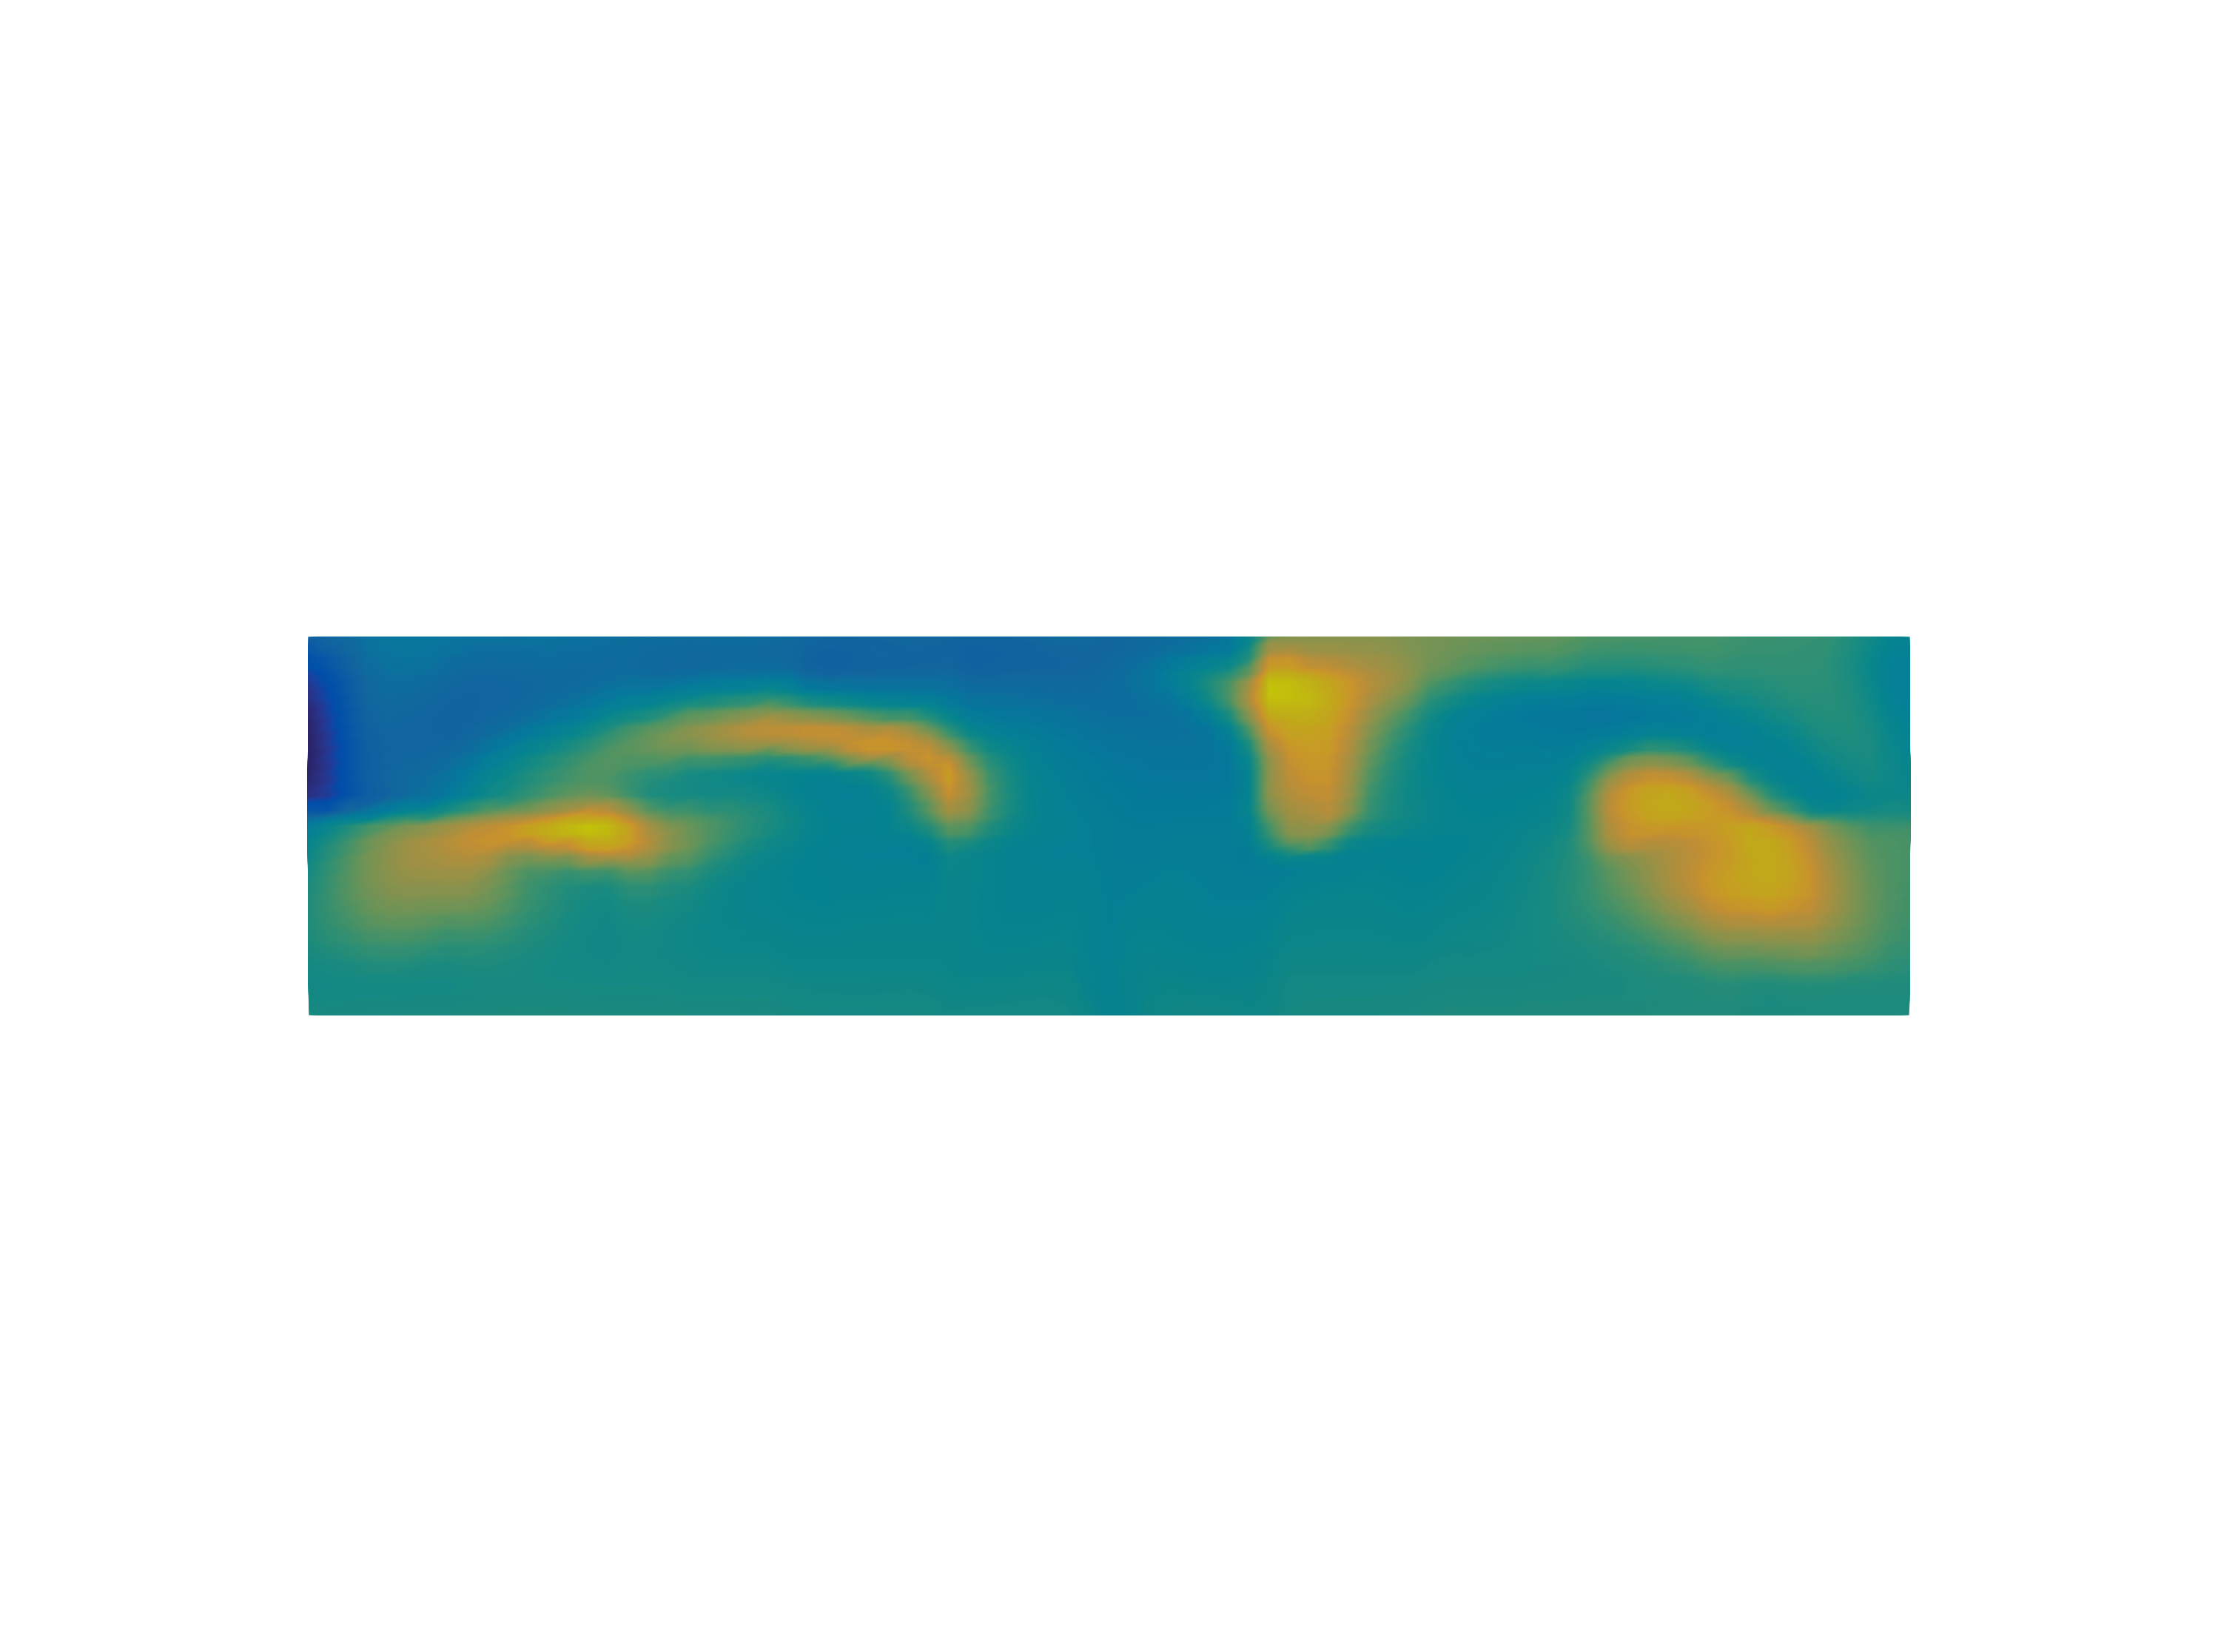
\includegraphics[width=\rasterimagewidth]{{../media/populations/application/print/alumina-influance-sur10-2.51-3.13}.png}}};
        \end{axis}
      \end{tikzpicture}
      \caption{Champ de concentration $c$ dans l'ACD de la cuve AP32 à
        $t = \num{10000}$ \si{\second}. De haut en bas, la température
        de surchauffe initiale est $\tsur = $ \numlist{1;2;5;10}.}
    \label{fig:dissolution-alumin-influence-sur}
  \end{center}
\end{figure}
